\section{Details of Experiments}

\subsection{Implementation environment} 
We implement our code based on Pytorch \footnote{https://pytorch.org/} and Transformers \footnote{https://github.com/huggingface/transformers}. The Python version for implementing the codes and constructing the dataset is Python 3.9.12. All pretrained code language models are automatically downloaded from Hugging Face \footnote{https://huggingface.co/models}. 

\subsection{Performance on the different types of the function calls}
\begin{table*}[ht]
\centering
\begin{tabular}{ccccccccc}
\toprule
\multirow{2}{*}{Task} & \multirow{2}{*}{Model} & \multirow{2}{*}{Context}  & \multicolumn{2}{c}{stdlib} & \multicolumn{2}{c}{in-project} & \multicolumn{2}{c}{third-party} \\
\cmidrule{4-9}
                      &                        &                          & EM      & EditSim   & EM    & EditSim        & EM         & EditSim \\
\midrule
Unidirectional        & CodeGen-MONO          & local context.            & 51.81   & 77.58     & 46.32 & 73.67           & 34.23         & 67.62   \\
                      &                        & +implementation\&usages  & 60.00   & 81.49     & 66.02 & 86.42           & 52.52         & 77.00   \\
                      & CodeT5-base            & local context            & 52.38   & 77.57     & 45.02 & 73.21           & 35.77         & 67.30   \\
                      &                        & +implementation\&usages  & 60.12   & 81.99     & 66.53 & 87.20           & 50.86         & 77.20   \\
\midrule
In-filling            & CodeT5-base            & local context            & 61.48   & 82.97     & 54.76 & 79.60           & 44.77         & 73.73   \\
                      &                        & +implementation\&usages  & 68.27   & 86.78     & 71.89 & 90.06           & 57.39         & 81.61   \\
\bottomrule
\end{tabular}
\caption{The performance of different types of the function calls on our new call argument completion dataset.}
\label{tab:types}
\end{table*}

The function definitions of the calls in our dataset may come from three sources: 
1) other files in the same project (in-project); 
2) third-party dependencies (third-party); and
3) the built-in standard libraries of Python (stdlib). 
We evaluate the model performance on these three types of functions using the same models from Table \ref{tab:fc_all}. 
The results are shown in Table \ref{tab:types}. 

We find that when using the local context only, the models perform best on the function calls defined in the standard libraries. 
This may be partly due to that the standard libraries are treated as the shared information between the training and test set, and partly due to that this type of functions constitutes a relative large amount of occurrences. 
Both of the facts make it easier for the models to pick up and generalize the patterns even if only the local context is available.

However, when using function implementation context and function usage context, the completion performance for in-project and third-party function calls greatly increased. 
Especially for in-project function calls, now their EM and EditSim numbers even surpass those of stdlib calls.
It provides yet another evidence for the importance of using in-project and cross-project information in models' generalizability cross projects for code tasks. 

\subsection{Exact match in the usages} 
\label{sec:saturate}
\begin{figure*}[bt]
\centering 
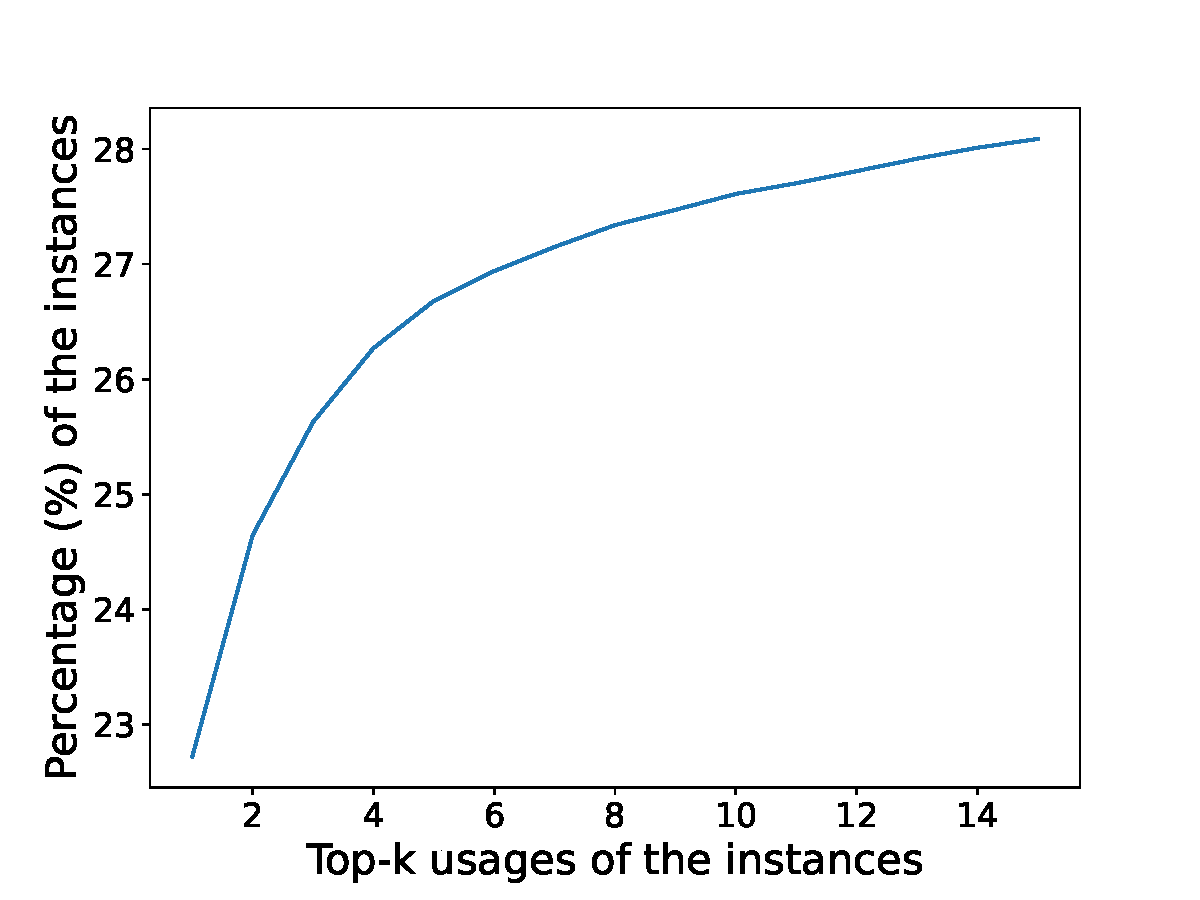
\includegraphics[width=0.5\linewidth]{fig/curve.pdf}
\caption{Percentage of function calls where at least one of their top-k usages shares the same arguments. Calculated from the \CallArgs validation set.}
\label{fig:curve}
\end{figure*}

We see from \Figref{fig:curve} that the coverage of exact argument matches in top-$k$ usages increases not much when $k > 6$. 
It partially explains the observations in \Tabref{tab:fc_length} that providing more numbers of usages does not necessarily bring benefit to the model performance.